\subsection{Verschillende leersnelheden}
In dit experiment bekijken we hoe de leersnelheid $\alpha$ het neurale netwerk be\"invloed. De leersnelheid $\alpha$ geeft aan hoe snel een netwerk van "gedachten" verandert. Een hogere leersnelheid betekent dat het netwerk zich sneller aanpast aan exceptionele gevallen, waardoor het sneller kan leren. Het gevaar hiermee is als $\alpha$ te hoog is, dat het netwerk zich teveel aanpast waardoor gemiddelde gevallen verkeerd worden beantwoord. Als $\alpha$ te laag is dan past het netwerk zich weinig aan aan veranderingen en leert het netwerk langzamer.

\begin{table}[ht]
    \centering
      $\begin{array}{c||c|c |}
        \alpha & \text{Aantal correct} & \text{Percentage \% correct} \\ \hline
        0.1 & 27 & 54 \\ \hline
        0.2 & 29 & 58 \\ \hline
        0.3 & 37 & 74 \\ \hline
        0.4 & 45 & 90 \\ \hline
        0.5 & 46 & 92 \\ \hline
        0.6 & 43 & 86 \\ \hline
        0.7 & 39 & 78 \\ \hline
        0.8 & 42 & 84 \\ \hline
        0.9 & 39 & 78 \\ \hline
        1.0 & 41 & 82 \\ \hline
      \end{array}$
    \caption{Aantal correcte antwoorden over 50 executies met verschillende leersnelheden}
    \label{tab:leersnelheden}
\end{table}

\begin{figure}[ht]
    \centering
    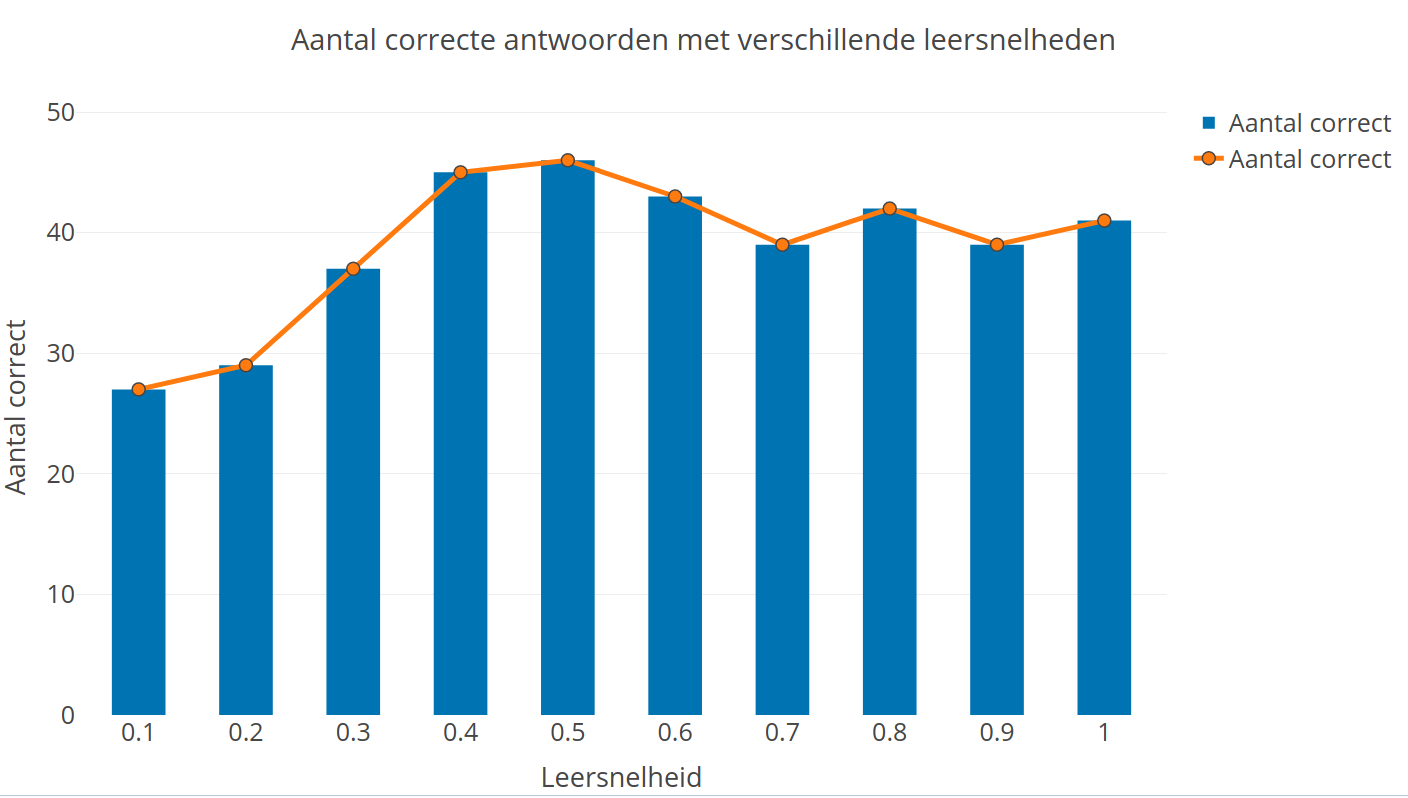
\includegraphics[scale=0.3]{graphs/leersnelheden.png}
    \caption{Aantal correcte antwoorden over 50 executies met verschillende leersnelheden}
    \label{fig:leersneheden}
\end{figure}

We zien in Figuur \ref{fig:leersneheden} dat er wel degelijk een piek is rond een $\alpha$ van 0.5 en dat hogere leersnelheden een lagere hoeveelheid correcte antwoorden geeft. Dit komt, zoals eerder gezegd, doordat hogere leersnelheden ervoor zorgen dat het netwerk zich meer aanpast aan exceptionele gevallen. Een $\alpha$ van 0.5 is groot genoeg dat het netwerk zich voldoende aanpast om zoveel mogelijk het correcte antwoord te geven en klein genoeg dat het exceptionele gevallen niet als de norm gaat zien.